% !TeX root = Logpp.tex
Given the design principals outlined in \autoref{sec:implementation} we now 
present the implementation of \projn\footnote{\projn sources available at 
\url{https://github.com/mrkmarron/logpp}} which realizes these goals in a logger 
for the \texttt{Node.js}~\cite{Node} runtime. It is possible to implement many 
of the features needed to satisfy our design goals as a library or using the 
native API extension bindings (N-API~\cite{NAPI}) but others require core 
runtime support. For these core changes we modify the ChakraCore JavaScript 
engine and core Node implementation directly.

\subsection{Implementation Overview}
The logging system is split into five major components that (1) manage the 
global logger states, message formats, and activities (2) the in-memory logger 
(3) the stage processor (4) the formatter (5) and finally the emitter. These 
components and the relations between them are shown in~\autoref{fig:arch} and 
explained in detail in the rest of the section. We will also use a running 
example in~\autoref{fig:runningExample} to illustrate various aspects of the 
system.

\begin{figure}
    \centering
    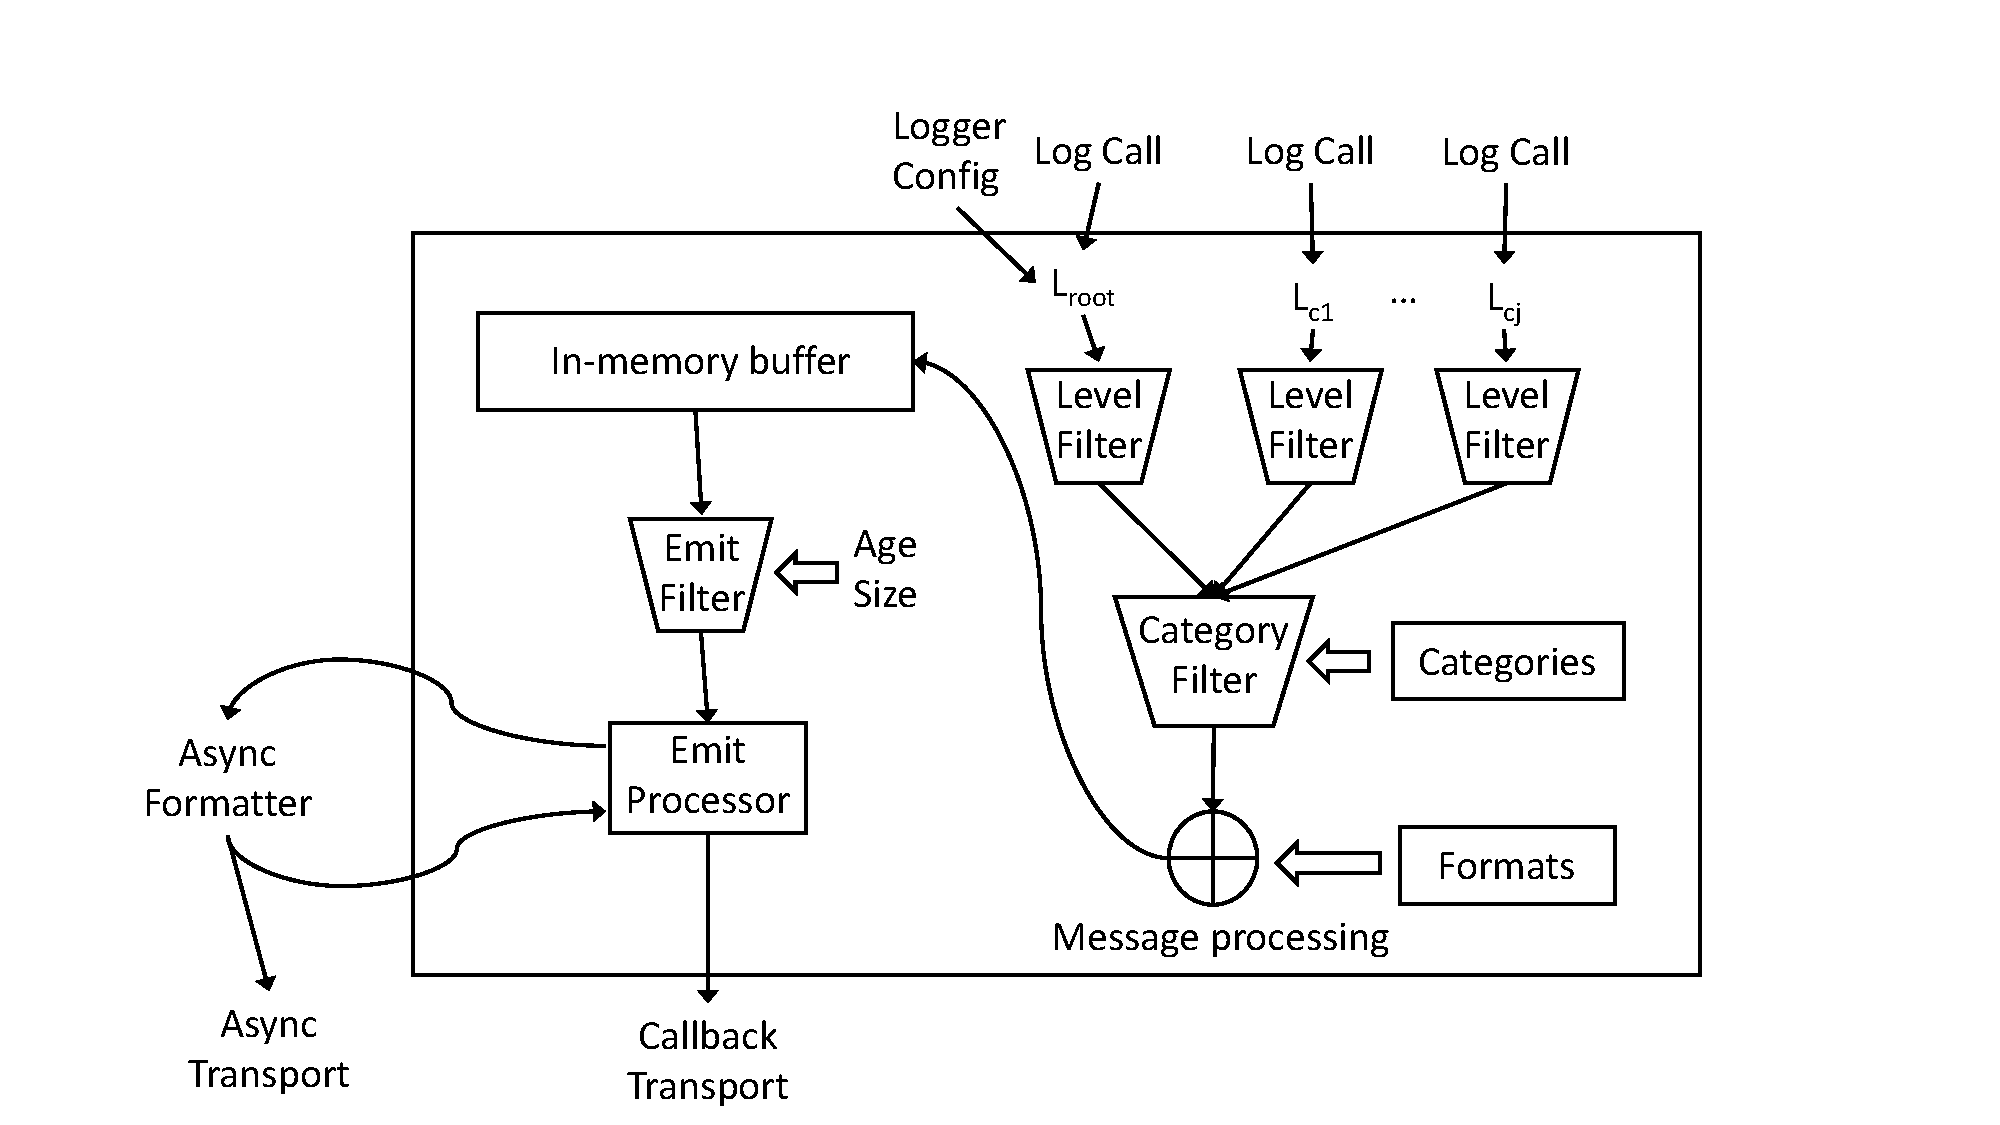
\includegraphics[width=0.5\textwidth,angle=-90]{Figures/ArchDiagram}
    \caption{Logger architecture}
    \label{fig:arch}
\end{figure}

\begin{figure*}[t]
\begin{minipage}[b]{0.47\textwidth}
    \lstinputlisting[language=JavaScript,basicstyle=\scriptsize]{Code/runningExample.js} 
    \caption{Main app code}
    \label{fig:appmain}
\end{minipage}
\begin{minipage}[b]{0.47\textwidth}
    \lstinputlisting[language=JavaScript,basicstyle=\scriptsize]{Code/runningExampleSub.js}
    \caption{Submodule code}
    \label{fig:appsub}
\end{minipage}
\caption{Running example}
\label{fig:runningExample}
\end{figure*}

\subsection{JavaScript Implementation}
\label{subsec:jsimpl}
\paragraph{Log State Manager}
\noindent
The first component we look at in the implementation is the global log state 
manager. This component is responsible for tracking all of the loggers that 
have been created, which is the root logger, the enabled logging levels + 
categories, and the message formats which have been defined. 

As seen in~\autoref{fig:arch} and the running example may be many loggers 
created in different parts of the application. One logger is created on line 
2 of the main application~\autoref{fig:appmain} while a second is created 
in the module \texttt{foo.js} in~\autoref{fig:appsub} which is included from 
the main \texttt{app.js} file. As stated in \emph{design principle 5} we 
do not want the included sub-module \texttt{foo.js} to be able to, unexpectedly, 
change the logging level for the main app (the call to \texttt{setOutputLevel} on 
line 9). We also want to allows the root logger to enable/disable log outputs 
from these subloggers. 

To support these features the \projn logger keeps a list of all created loggers 
and a special \emph{root logger} which is the first logger created in the main 
module of the application. When updating logging levels or creating a new logger 
we check if action is comming from the root logger and, if not, either convert 
the call to a \texttt{nop} or look at the root logger configuration to see if 
we need to override any parameters. These features cover the needs of controlling 
logging from multiple modules as desribed in \emph{Design Principle 5}.

In our running example the state manager will intercept the creation of the logger 
on line 2 in \texttt{foo.js}. Since the logger created here is not the root logger
the state manager will intercept this construction, set the in-memory log level to 
the overridden \texttt{WARN} level instead of the default value of \texttt{DETAIL}, 
prevent the modification of the \emph{emit-level} or the output sink, and will 
store the newly created logger in a list of sub-loggers. 

Tracking the list of all created sub-loggers also allows a developer to share a 
single logger between several files in the same module. The name parameter in the 
logger constructor is keyed with the logger and, if the same key is used in multiple 
places, the same logger object will be returned.

Finally, the state manager is responsible for maintaining information on the current 
\emph{emit level}, the enabled/disabled categories, and the sublogger override information. 
Each logger has an independent level at which it can write into the in-memory log but 
the state manager maintains a global set of enabled/disabled categories which each logger 
uses and a global logging level for eventual emit processing. Only the root logger is 
allowed to update the categories and emit levels. 

In our running example the main application has a log statement on lines $12$ and $14$ 
that are in the \texttt{Perf} category and will put a message with the current walltime 
in the log. As the first log statement happens before the \texttt{Perf} category has 
been enabled it will not be processed. However, after enabling the \texttt{Perf} category 
on line $13$ the log operation on line $14$ will be processed and result in a message 
being saved to the in-memory log.

\paragraph{Message Formats}
\noindent
To improve performance and enable the log output to be easily machine parsed we 
adopt a \emph{semantic logging} approach where the log call copies the format 
information and message arguments to a secondary location instead of formatting them 
immediately. This implementation choice supports the needs of \emph{Design Principle 2}.
Since the copy operation is very low cost this minimizes the 
performance impact on the main thread and allows the formatter to build up a 
parser for all the messages it emits which can be later used to parse the log. 
Modern software development also favors the use of consistent styles and data 
values in the log. Thus, \projn encourages developers to split the logging 
action into two components:
\begin{itemize}
\item Format definition using the \texttt{addFormat} method which takes a format 
string or JSON format object, processes it into an optimized representation, 
and then saves it for later use.
\item Format use in a log statment which takes a format identifier and a list of 
arguments, and then, processes them.
\end{itemize}

In addition to programtically processing single log formats, as shown on line 3 
in~\autoref{fig:appmain}, we also allow the programmer to load formats in bulk 
from a JSON formatted file. This allows a team to have a unified set of logging 
messages that can be loaded/processed quickly on startup and then used repeatedly 
throughout the applications execution. Once loaded all format objects are saved 
in the \emph{formats} component in~\autoref{fig:arch} where they can be loaded 
as needed for processing a log statement.

The format for a logger message is:
\begin{lstlisting}[language=JavaScript,basicstyle=\scriptsize]
{
  formatName: string, //name of the format
  formatString: string, //raw format string
  formatterEntries: {
    kind: number, //tag indicating the entry kind
    argPosition?: number, //position in argument list
    expandDepth?: number, //JSON expand depth
    expandLength?: number //JSON expand length
  }[]
}
\end{lstlisting}

This representation allows us to quickly scan an process the arguments as 
described in the \emph{Message In-Memory Processing} section. The kind 
information is used for both identifying what type of value is expected 
when formatting an argument, e.g. \texttt{number}, \texttt{string}, etc., 
but we also use it to support \emph{format macros}.

To support the easy/efficient logging on a number of common values that 
are not easily (or cheaply) computable we provide \emph{format macros}. 
Classic examples include adding the current walltime or the hostname as 
part of a log message. In JavaScript these require explicitly calling 
expensive compund API sequences \texttt{new Date().toISOString()} or 
\texttt{require('os').hostname()}. Instead we allow a developer to use 
special macros \texttt{\#walltime}, as seen on line 11 in~\autoref{fig:appmain}, 
or \texttt{\#host} in their format 
strings and then the logger has optimized internal paths to get the needed 
values. In these cases the \texttt{kind} field is set to the enumeration 
for the macro and the \texttt{argPosition} is undefined. The list of supported 
macro formatters includes:
\begin{itemize}
  \item \#host -- name of the host
  \item \#app -- name of the root application
  \item \#logger -- name of the logger
  \item \#source -- source location of log statment (file, line)
  \item \#wallclock -- wallclock timestamp (ISO formatted)
  \item \#timestamp -- logical timestamp
  \item \#request   -- the current request id (for http requests)
\end{itemize}

A common logging practice is to include raw objects, formatted as JSON, into the 
message. This is a convinient way to include rich data into a message but can 
lead to unexpectedly large logging loads when, what the developer expected to 
be a small object, turns out to be quite large. To prevent this we have a specialized 
JSON-style processor that will bound the depth/length of object expansion during 
formatting. The \texttt{expandDepth} and \texttt{expandLength} arguments provide 
control over this depth/length and can be adjusted in the format string when a 
developer want to capture more (or less) information than what is provided by the 
defaults.

\paragraph{In-Memory Message Processing}
\noindent
The in-memory buffer is implemented as a linked-list of block structures:
\begin{lstlisting}[language=JavaScript,basicstyle=\scriptsize]
{
  tags: Uint8Array,
  data: Float64Array,
  strings: string[],
  properties: map<number, string>
}
\end{lstlisting}

To allow efficient marshalling of the data from our JavaScript logger frontend 
to the C++ N-API code that handles the formatting we encode all values into 
$64$bit based representation (stored in the \texttt{data} property). We use a set 
of enumeration \texttt{tags} (stored in the \texttt{tags} property) to track 
what kind of value the corresponding $64$bit value represents. We have special 
handling for string and object properyt values, described below, that use the 
\texttt{strings} array and \texttt{properties} map to index and keep alive these values.

When implementing a sematic logging system the key invariant that needs to be 
preserved is that the values of each argument must not be changed between the 
time when the log call happens and when the argument is processed for 
formatting. Certain values including booleans, numbers, and strings, are 
immutable according to the language semantics so we can just copy the 
references directly into our in-memory array. However, in cases where the 
argument is a mutable object we must take explicit actions. A simple solution 
would be to JSON \texttt{stringify} the argument immedaitely, and while this 
prevents mutation and allows semantic formatting, it comprimises possible 
performance gains we are looking for. Instead we recursively flatten the object 
into the in-memory buffer with the code shown here:

\lstinputlisting[language=JavaScript,basicstyle=\scriptsize]{Code/flatten.js}

This code represents the transition from the \emph{formats} and \emph{arguments} 
inputs into the \emph{in-memory buffer} shown in~\autoref{fig:arch}. This code 
starts off by checking if we are either in a cycle or the depth bound has been 
reached. If either of these occour we put a special tag, \texttt{CycleTag} or 
\texttt{DepthBoundTag} respectively, into the tags array and return. If not we 
continue with the pre-order traveral of the object graph by updating the cycle 
info, adding the special \texttt{LParenTag} to the buffer, and enumerating the 
object properties. For each property we check if the length bound is met, adding 
the special \texttt{LengthBoundTag} and breaking if needed, if not we add the 
property and value information to the in-memory buffer. The property value \texttt{p} 
is a special string value which is very likely to be repeated so we use a map 
from properties to unique numeric identifiers to compress and convert them into 
a number which can be stored in the \texttt{data} component of the in-memory buffer 
via the \texttt{addPropertyEntry} function. The value associated is recursively 
processed via the \texttt{addGeneralEntry} call which switches on the type of the 
value, booleans and numbers are converted directly to \texttt{Float64} representations, 
strings are mapped by index in the \texttt{strings} array, and \texttt{Date} objects 
are converted to $64$bit timestamps using the \texttt{valueOf} method. Similar to 
standard JSON formatting other values are simplified but, instead of just dropping 
them, we use a special \texttt{OpaqueValueTag}. After all the properties have 
been processed we update the cycle tracking information and add a closing 
\texttt{RParenTag}.

\begin{figure}
    \centering
    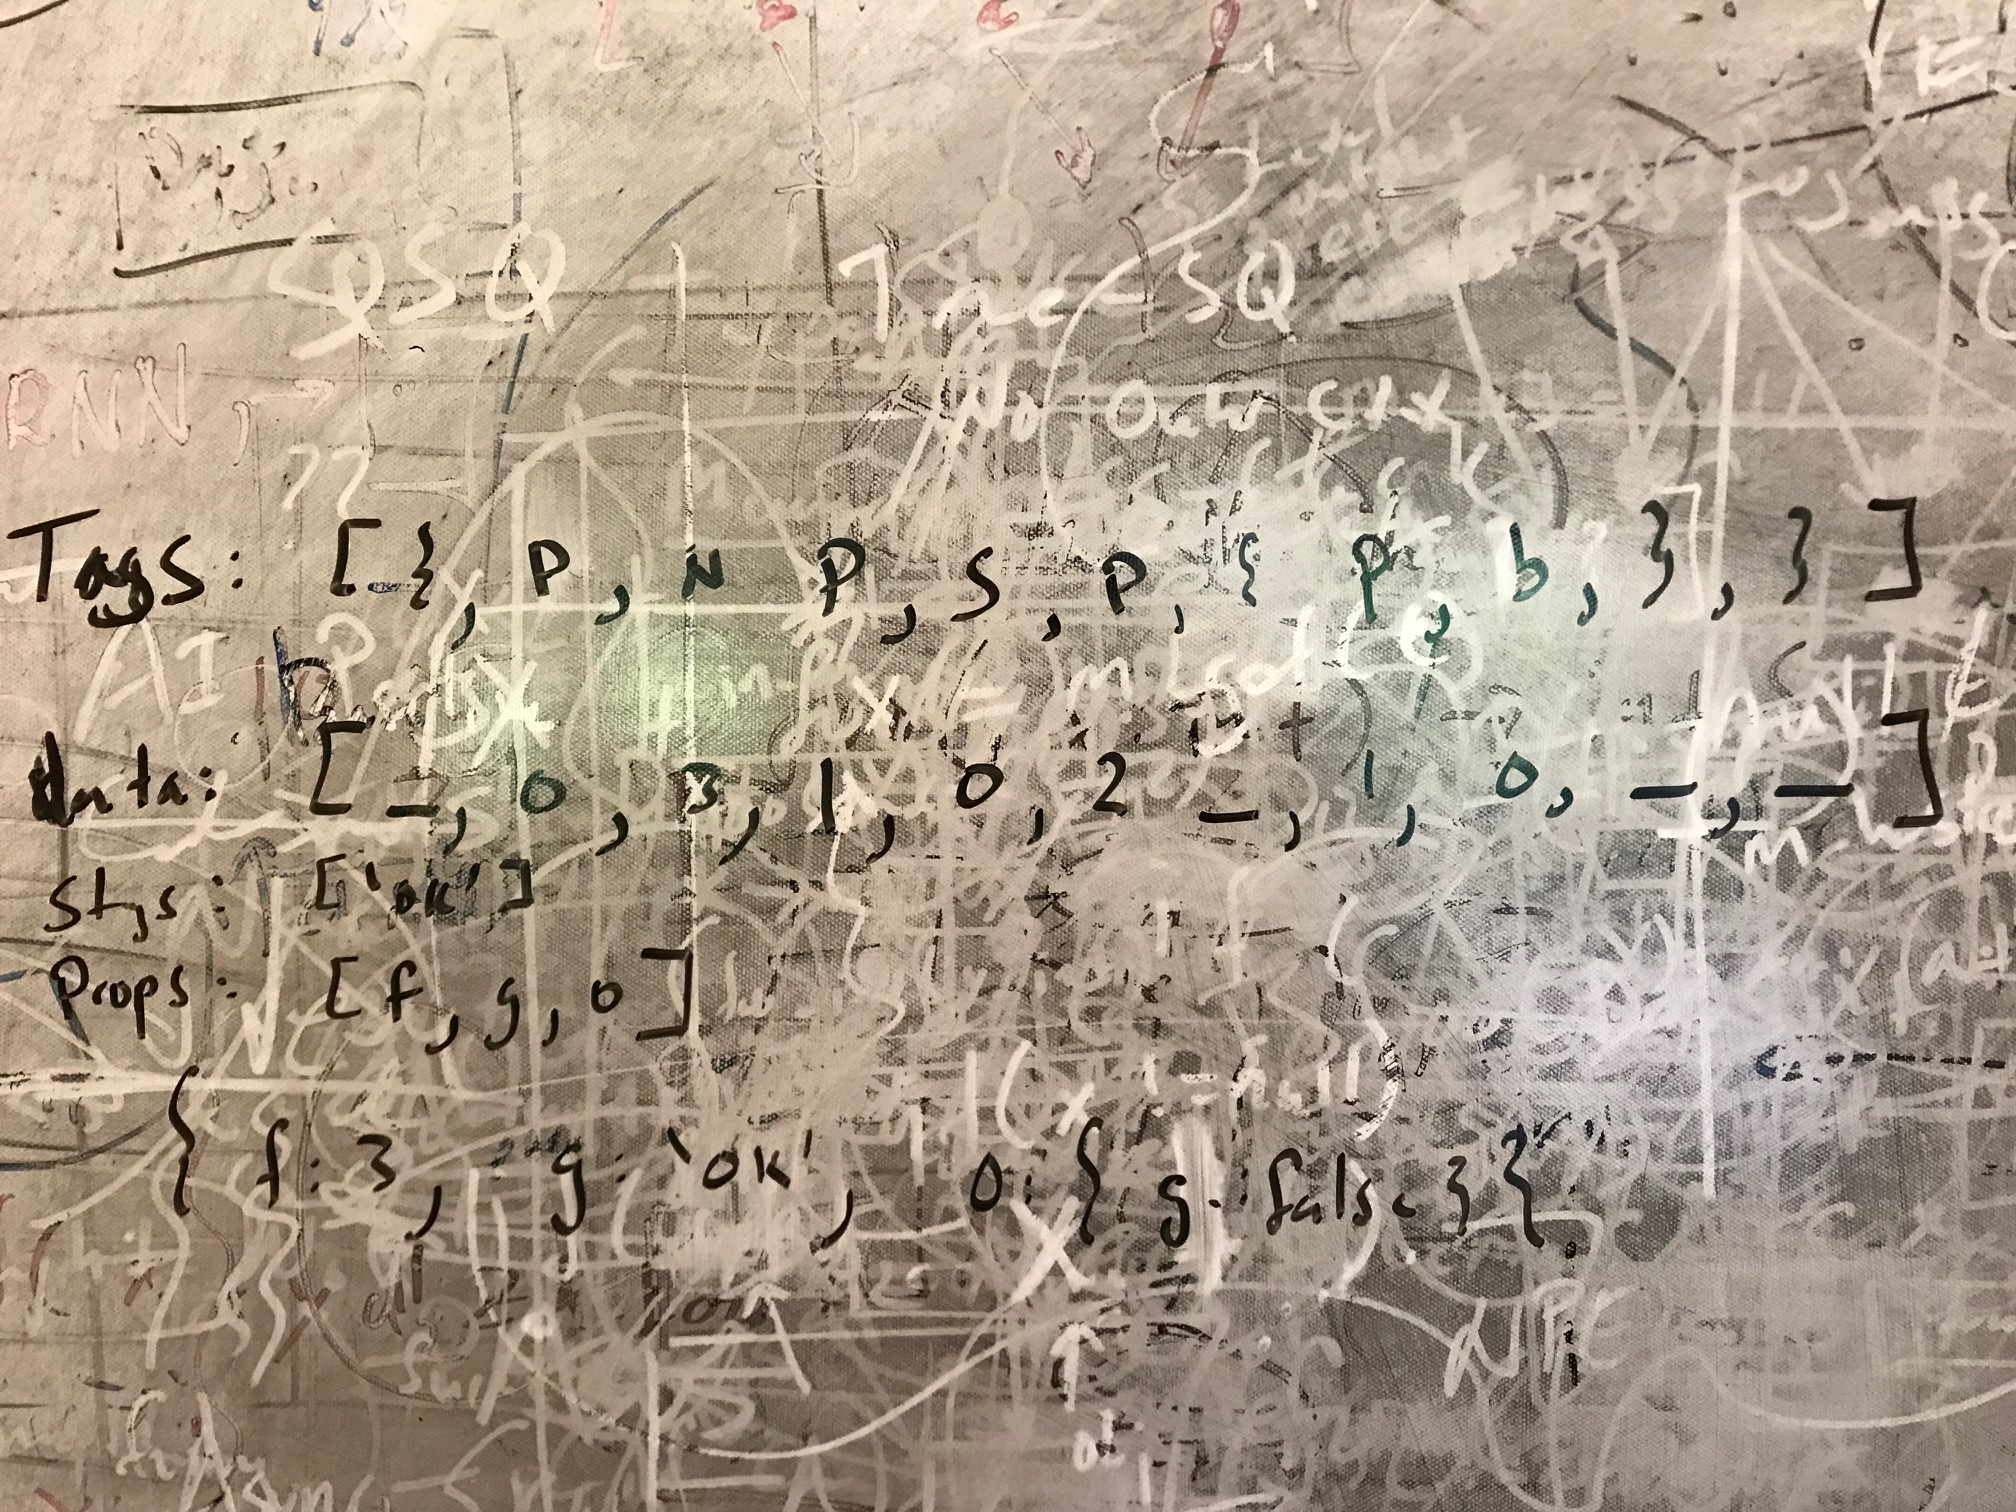
\includegraphics[width=0.5\textwidth]{Figures/InMemoryExample}
    \caption{In-Memory buffer processing example}
    \label{fig:inmemory}
\end{figure}

To illustrate how this code works in practice consider the case of processing the 
object argument:

\begin{lstlisting}[language=JavaScript,basicstyle=\scriptsize,numbers=none]
{
  f: 3,
  g: 'ok',
  o: { g: false, id: (x) => x }
}
\end{lstlisting}

The resulting state of the in-memory buffer is shown in~\autoref{fig:inmemory}. 
In this example we can see how the object structure has been flattened into 
the buffer with the \lstinline!'{'! and \lstinline!'}'! tags denoting the bounds 
of each object. Each of the properties has been registered in the map (with a fresh 
numeric identifier) and this is stored in the \texttt{data} array. For example the 
property \lstinline!g! is mapped to $1$ and in both occournces in the object 
structure the entry in the \texttt{tags} array is set to \lstinline!'p'! for 
property and the value in the \texttt{data} array is set to match the corresponding 
numeric identifier $1$. The numeric and boolean values are mapped in the obvious 
way, directly for the number and to $0$/$1$ for the boolean with the appropriate 
tag values set. Similar to the properties the string value \lstinline!'ok'! is 
mapped to an integer index, index $0$, in the \texttt{strings} array. Finally, 
since functions are not serializable, the value associated with the \lstinline!id! 
property is dropped and we simply store the \texttt{OpaqueValueTag} (\lstinline!'?'!) 
in the corresponding position of the \texttt{tags} array.

\paragraph{Message Staging}
\noindent
The in-memory design allows us to support \emph{Design Principle 3} by buffering a 
window of high detail messages, in case they are needed for diagnostics, and then 
asynchronously filtering and flushing out high level telemetry messages to stable 
storage. Whenever a message is written into the in-memory buffer we do a simple 
\texttt{writeCount} check, to limit the flush rate, on the number of messages written 
since the last flush if more than this threshold have been written we schedule an 
asynchronous flush process on the event-loop. The flush code filters the messages 
based the current \emph{emit} level and processes all messages that exceed the 
specified \texttt{age} and \texttt{memory} thresholds. The implementation of the 
filter/process step from~autoref{fig:arch} is:

\lstinputlisting[language=JavaScript,basicstyle=\scriptsize]{Code/process.js}

This code works by looping over the messages in the in-memory buffer passed in, 
\lstinline!buff!, and will either process all the messages in the buffer or 
stop when the \lstinline!ageCheck! or \lstinline!sizeCheck! conditions no longer 
hold. These conditions check if a message is older than the specified 
\lstinline!age! measured from the current time and that overall memory 
consumption is less than \lstinline!size! respectively. The intent behind the 
age limit is to prevent the overly eager discarding of log messages that might 
be relevant for debugging. While the intent behind the size condition is to ensure 
that an application which has a heavy burst of logging will not cause excessive 
memory consumption even if the messages have not aged out yet.

If an issue, currently defined as an unhandled exception or an exit with non-zero code, 
is encountered during execution the logger will immediately flush all the logger 
messages to the serializer regardless of age or level. This ensures that there is maximal 
detail for the developer when trying to diagnose the issue. \projn also supports 
programtic force-flushing of the log, with the \texttt{forceFlush} method, for cases where there 
is an issue that the developer wants to understand but does not result in a hard failure. 

\paragraph{Emit Callback}
\noindent
Once the in-memory buffer has been processed the logger passes the filtered set of 
log messages to the background \emph{asynchronous formatter} (described in~\autoref{sec:nativeimpl}) 
which, when formatting is complete, will default to invoking a callback into the 
JavaScript application. For common cases we provide the simple default callback that 
writes to stdout or, if a \texttt{stream} is provided, to write the logs out through 
it. In the most general case a user can configure the logger with a custom callback, 
called with the formatted log data, which can perform any desired post processing and 
send the data to arbitrary (or multiple) sinks.

\subsection{Native Formatting and Optional Native Emit}
\label{sec:nativeimpl}
Once the in-memory buffer has been processed the logger passes the filtered set of 
log messages to the background \emph{asynchronous formatter} in~\autoref{fig:arch} which 
is implemented in Native code using the N-API~\cite{NAPI} module. The direct 
implementation of this module does not have any low-level hooks into the GC of 
the host JavaScript engine so we must fully copy any data needed before starting 
the background processing (a limitation we discuss relaxing in~\autoref{sec:runtimesupport}). 
However, once the data copy is done the formatting thread can run completely in parallel 
to the main JavaScript thread and can use an optimized C++ formatting implementation. This 
not only allows us to reduce the overall formatting cost but also to move this cost 
entrirely off the hot-path of JavaScript exection.

In addition to background formatting \projn also supports background emitting, 
shown as the \emph{background emit} block in~\autoref{fig:arch}, of 
logging data to files, stdout, or a remote url provided at configuration time. This 
allows us to skip re-marshalling the formatted data into a JavaScript string as well 
as reduces the number of JavaScript callbacks and associated time spent on the 
main thread there. 

By default the native formatter produces JSON compliant output. However, this 
can be verbose to send and store so we offer serialization format and compression 
options for optimization. In addition to JSON a user can configure the logger 
to format to a simple binary encoding format which is not human readable but 
substantially more compact (\todo{HOW MUCH}) and computationally efficient to 
encode into. With either format the logger can also be configured to compress the 
formatted data as well using the \texttt{zlib} library already included in 
Node.js core.

\subsection{Logging APIs}
As described in \emph{Design Principle 4} there are frequent cases where a 
simple call to a log statement is insufficient and a developer would normally 
need to add explicit logging-specific logic. To avoid this clutter, and potential 
source of errors, we provide a richer set of logging primitives:
\begin{itemize}
  \item \emph{conditional logging} which allows a user to specify a condition 
  that guards the execution of the log statement. This eliminates the need to 
  introduce logging specific control flow into the code.
  \item \emph{child loggers} which create a logger object that prefixes all log 
  operations called on it with a specified value (used frequently for logging in a 
  subcomponent).
  \item \emph{request specific logging} which allows a developer to set a different 
  logging level and enabled categories for a specific \texttt{RequestID}. This is a 
  common need for cloud-based applications, particularly when participating in a 
  smapling distributed logging system~\cite{distlogger}.
  \item \emph{interval bounding} which writes a log message at the start of an interval 
  and accepts a payload which can be accessed when writing the end event for the interval. 
  This allows the transparent, instead of explicit, propagation of the needed data between 
  the related log actions.
\end{itemize}

An example of the utility of these loggers, conditional logging, is in our introductory 
example from~\autoref{fig:introExample} where the condition on line 14 was introduced 
soley in support of the logging output. Using our conditional logging APIs this condition 
and log combo can be replaced by a single line \lstinline{logger.warnIf(!ok, "Error...")}.

\subsection{Custom Runtime Implementation}
\label{sec:runtimesupport}
The previous sections described the \projn logger as it can be implemented as a purely 
userspace module in Node.js and as it is publically available. However, there are 
issues, optimizations, and improvements that require close interaction with the 
runtime and/or compiler. This section describes these and how we have explored their 
implementation in Node-ChakraCore, the version of Node.js running the ChakraCore 
JavaScript engine from Microsoft. 

\paragraph{Format and Mutability Checking}
\noindent
Two programming errors that are specific to logging are mismatched arguments used 
for the provided format specifiers and accidental side-effects in logging related 
code. \projn takes the view that logger calls should, if all possible, not cause 
an application failure and instead note invalid arguments in the output formatting. 
Previous work~\cite{tyepcheckprintf} has shown how to include static type 
checking for log arguments as well. A similar approach can be taken to combine 
work on purity analysis~\cite{purity1,purity2} to ensure that any code executed 
in a log statement does not modify externally visibile state. These features require 
at least support in a linter, such as \emph{eslint}~\cite{eslint}, or integration 
with the language itself.

\paragraph{Zero-Cost Disabled Logging}
\noindent
Developers have low trust that logging disabled by setting levels or categories 
will not continue to impact performance. Thus projects often experience frequent 
code churn as logging is added for a task and then removed afterword to avoid 
performance issues. This wastes substantial developer time, creates opportunities 
to introduce accidental regresssions, and prevents the development of a comprehensive 
base of logging code in an application. 

To ensure that disabled log statements truely are zero-cost requires cooperation 
with the language spec and the JIT. To avoid parasitic costs of evaluating log 
arguments that will be immediately discarded, like line 8 in~\autoref{fig:introExample}, 
we must lazily evaluate them after the level, category, and (optional) condition 
checks have completed. We also want the JIT to be particularly aware of the guards 
around log statements, aggressively optimizing the guard paths, and performing 
dead-code-elimination or motion on computations that are only used for log arguments.

\paragraph{Fast Handling for Strings and Properties}
\noindent
Strings and JavaScript object properties are frequently occouring values in 
parts of a log message. If we are limited to a purely JavaScript and N-API 
interface we are forced to treat the properties as strings and we must 
definsively copy the strings wihen processing them in the \emph{message staging} 
process otherwise the JavaScript engine GC may move them while the formatter is 
accessing the underlying memory creating a data race and corruption. 

Modern JavaScript engines use internal numeric \emph{Property Identifiers} 
instead of strings when dealing with object properties. These are much more 
compact and efficent to process for both the engine and, in our logger, would 
allow us to copy a single integer into our in-memory buffer instead of creating 
our own indexing scheme. Thus, we expose a new 
JavaScript API, \texttt{loggerGetPropertyId(propertyString)}, which returns the 
internal numeric identfier for a property string to use in the message staging. 

To avoid costs associated with data marshalling and copying string data 
in the formatter we need to introduce 3 APIs. The first is a pair of 
methods, \texttt{loggerRefString} in JavaScript which will tell the JavaScript 
engine that it needs to reference count, flatten, and intern a string (if needed) 
with a unique numeric value (which is returned), and \texttt{loggerReleaseString} 
which decrements the reference count and unpins the string if needed. These 
allow us to avoid copies when marshalling the string in the \emph{message staging} 
phase. As various JavaScript engines use different internal widths for characters 
we we add a \emph{getNativeStringCharSize} method to determine if strings 
are \texttt{utf8} or \texttt{utf16} encoded. In combination with \texttt{getRawBytes} 
and \texttt{createStringWithBytes} methods this allows us to avoid any encoding 
conversions when formatting and creating strings. 

\paragraph{Priority Aware I/O Mangement}
\noindent
The final optimization we look at that requires runtime support is to ensure 
that logging related I/O and computation do not interfere with code high-priority 
code responding to user actions. In our implementation the msessage staging 
and uploading of formatted log data is done on the UV event loop. This loop does 
not have any notion of priority so we may accidentally block code responding 
to a user action with code that is processing log data. To avoid this we could 
add a special \emph{log work queue} to the existing Node event loop processing 
algorithm~\cite{nodeeventloop} but we believe that the notion of priority is 
fundamentally valuable and should be added to Node explicitly~\cite{asyncnode}. 
This \emph{priority promise} construction makes it trival to add logging related 
callbacks at a background task level (perhaps with a small time-limit) to ensure 
that logging activities are completed in a timely manner without impacting user 
responsiveness.






